\section{Дискретная математика}

\subsection{Частично упорядоченные множества}
$(M, \le )$ - Чум, его войства:
\begin{itemize}
	\item рефлексивность $\forall x \in M: x \le x$
	\item антисимметричность $\forall x,y \in M : x \le y \wedge y \le x \rightarrow x = y$
	\item транзитивность $\forall x,y,z \in M : x \le y, y \le z \rightarrow x \le z$
\end{itemize}
\vspace{1em}
Элементы \textbf{несравнимы}, когда $x \cancel{\le} y, y \cancel{\le} x$
\subsubsection{Диаграмма Хасса}
$a \prec b$
\begin{itemize}
	\item $a \le b, a \neq b$
	\item $a \le c \le b \rightarrow a =c \vee c = b$
\end{itemize}
Число отношений порядка на $\{1 \dots n\}$ равно $n!$ 
\subsection{Графы}
\subsection{Голосарий}
\begin{itemize}
	\item Изоморфизм. Два графа называются изоморфными, если существует перестановка вершин, при которой они совпадают. Иначе говоря, два графа называются изоморфными, если существует взаимно-однозначное соответствие между их вершинами и рёбрами, которое сохраняет смежность и инцидентность (графы отличаются только названиями своих вершин).
	\item Маршрут в графе — это чередующаяся инцидентных последовательность вершин и рёбер 
	\item Простая цепь в графе — маршрут, все рёбра которого различны. 
	\item Цикл — замкнутая цепь.
	\item Простой цикл — цикл, не проходящий дважды через одну вершину.
	\item Гамильтонов путь — простой путь в графе, содержащий все вершины графа ровно по одному разу.
	\item Гамильтонов цикл — простой цикл в графе, содержащий все вершины графа ровно по одному разу.

	\item Двудольный граф — это граф  $(V,E)$, такой, что множество вершин V разбито на два непересекающихся подмножества $V_{1}$ $V_{2}$, причём всякое ребро E инцидентно вершине из $V_{1}$ и вершине из $V_{2}$\\ \textbf{Теорема Кенига} Граф $G$ является двудольным тогда и только тогда, когда все циклы в графе $G$ имеют чётную длину. \\ Следствие - алгоритм проверки на двудольность:  за один проход в глубину. На каждом шаге обхода в глубину помечаем вершину. Допустим, мы пошли в первую вершину — помечаем её как 1. Затем просматриваем все смежные вершины, и если не помечена вершина, то на ней ставим пометку 2 и рекурсивно переходим в нее. Если же она помечена и на ней стоит та же пометка, что и у той, из которой шли (в нашем случае 1), значит граф не двудольный. 
	\item Лемма о рукопожатиях — положение теории графов, согласно которому любой конечный неориентированный граф имеет чётное число вершин нечётных степеней. $$\sum_{v\in V} \deg(v) = 2|E|$$
	\item Планарный граф — граф, который может быть изображён (уложен) на плоскости без пересечения рёбер. \\ \textbf{Теорема Понтрягина — Куратовского}. Граф планарен тогда и только тогда, когда не содержит подграфов, стягивающихся в $K_5$ или $K_{3,3}$.
	\begin{figure}[H]
    \centering
    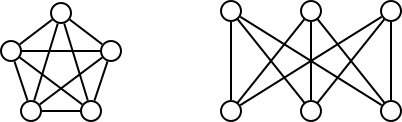
\includegraphics[width=0.5\linewidth]{k33andk5.png}
	\end{figure}
\end{itemize}

\subsection{Булева алгерба}
\subsubsection{Правило резолюций}
\begin{equation}
	\cfrac{A \vee B, \neg A \vee C}{B \vee C}
\end{equation}

\clearpage